\documentclass{ees}

\newgeometry{twoside=false,left=20mm,right=40mm,top=20mm,bottom=40mm}

\newlist{bulletlist}{itemize}{1}
\setlist[bulletlist]{
  partopsep=0pt,
  parsep=0pt,
  itemsep=0pt,
  label=\textbullet
}

\RedeclareSectionCommand[afterskip=0pt plus 1pt,runin=false]{section}
\RedeclareSectionCommand[afterskip=0pt plus 1pt,runin=false]{subsection}
\RedeclareSectionCommand[beforeskip=0pt plus 1pt, afterskip=0pt plus 1pt,runin=false]{subsubsection}
\RedeclareSectionCommand[beforeskip=0pt plus 1pt]{paragraph}
\setkomafont{section}{\normalfont\sbseries\large}
\setkomafont{subsection}{\normalfont\sbseries}
\setkomafont{subsubsection}{\normalfont\itshape}
\setkomafont{paragraph}{\normalfont\itshape}

\setcounter{tocdepth}{1}
\DeclareTOCStyleEntry[
  indent=0pt,
  beforeskip=\baselineskip,
  entrynumberformat=\@gobble,
  entryformat=\sbseries,
  numwidth=2em,
  linefill=\hfill,
  pagenumberbox=\pnumbox,
  pagenumberformat=\sbseries
]{tocline}{chapter}

\hyphenation{Musik-archiv}


\begin{document}

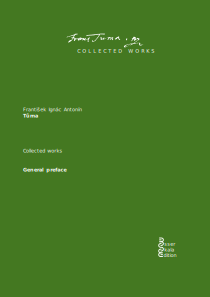
\includepdf{cover_general_preface.pdf}
\pagenumbering{arabic}
\setcounter{page}{1}

\tableofcontents

\chapter{General preface}

\textit{František Ignác Antonín Tůma: Collected works} (FIAT:CW) is an edition project that will make Tůma’s music available in modern editions. Simultaneously, it provides the source code used for typesetting the scores, thereby establishing a digital corpus of Tůma’s works that follows FAIR principles.

For more information, we refer the reader to our thematic catalogue of Tůma’s works, which is currently under development (\href{https://www.frantisek-tuma.at/}{https://www.frantisek-tuma.at/}). TumW numbers are cited from this catalogue.


\section{Editorial guidelines}

(In general, FIAT:CW follows the \href{https://edition.esser-skala.at/about/editorial-guidelines/}{editorial guidelines} for the Edition Esser-Skala, which are reproduced below.)


\subsection{Prefatory material}

Prefatory material comprises the title and copyright page. In addition, the full score also contains a critical report and table of contents.


\subsubsection{Title page}

The \textit{title page} (p. i) includes the following information:
\begin{bulletlist}
  \item a header with the composer's last name and the project title
  \item the composer's full name (last name printed in red)
  \item the title of the work (bold)
  \item a subtitle (if applicable)
  \item the catalog of works number
  \item the scoring
  \item the score type (e.g., “Full Score”, “Violino I”; use modern Italian names).
  \item the full logo of the Edition Esser-Skala
\end{bulletlist}

The \textit{scoring} lists all vocal parts and instruments:
\begin{bulletlist}
  \item Individual instruments are separated by commas (e.g., “S, vla, org”).
  \item An Arabic numeral prefix indicates the number of each instrument (e.g., “2 vl”).
  \item The pitch of transposing instruments is given in parentheses (e.g., “timp (C–G)”).
  \item Solo and chorus vocal parts are distinguished (e.g., “S, A (solo), S, A, T, B (coro)”).
  \item Instruments that are not available in all sources or have been added by the editor are surrounded by brackets (e.g., “[2 fl]”).
\end{bulletlist}

The \textit{copyright page} (p. ii) includes:
\begin{bulletlist}
  \item the copyright statement (CC BY-SA 4.0)
  \item an indication of used software and fonts
  \item contact details (email address)
  \item a link to the GitHub repository
  \item the current version, date, and SHA1 of the git repository
\end{bulletlist}


\subsubsection{Critical report}

The critical report (p. iii et sqq.) consists of three sections: abbreviations, sources, and commentary.

\paragraph{Abbreviations}
This section contains a table of used abbreviations. Instruments are abbreviated according to \href{https://opac.rism.info/scoring-abbreviations}{RISM}.

\paragraph{Sources}
This section describes the used sources of a given work. Each source is labeled with a bold capital letter (indicating the source category) followed by an index number:
\begin{bulletlist}
  \item \A{} – autograph manuscripts
  \item \B{} – other manuscripts used for the edition
  \item \C{} – prints used for the edition
  \item \D{} – manuscripts not used for the edition
  \item \E{} – prints not used for the edition
\end{bulletlist}

Within each category, sources are labeled in order of importance.

For each source, the following information is included:
\begin{bulletlist}
  \item RISM library siglum and shelfmark
  \item source category
  \item indication whether this source represents the principal source
  \item date (optional)
  \item RISM identifier (optional)
  \item link to digital version (optional)
  \item license
  \item notes (optional)
\end{bulletlist}

\paragraph{Commentary}
Each edition is based upon a single principal source, which is explicitly identified. Any substantial difference between the edition and the principal source is indicated with an asterisk in the score and reported in this section as an editorial \textit{emendation}.

However, the following elements are \textit{tacitly} modernized or standardized (see below for details): Tempo indications, instrument names, clefs, accidentals, beaming and stem directions, rests, placement of dynamics/slurs/ties, treatment of shorthand notations, bar numbering, bar lines, and repeats.

The table of emendations comprises the following columns:
\begin{bulletlist}
  \item movement (only if there are several movements in the work)
  \item bar number
  \item staff
  \item description
\end{bulletlist}

The following conventions apply to the commentary:
\begin{bulletlist}
  \item Keys are given with a capital letter for major or minor keys (e.g., “C minor”). Sharp and flat are spelled out with a hyphen (e.g., “B-flat major”).
  \item Notes are counted by ordinal numbers and written as symbol (e.g., “1st \quarterNote”).
  \item Helmholtz pitch notation is applied, with symbols for sharp, flat, and natural signs, and order name–accidental–octave (e.g., “\sharp c′”).
  \item Rests are written as symbol.
  \item A sequence of pitches is separated by en dashes (e.g., “c′4–d′8–e′8”)
  \item Chords are spelled with a plus sign between pitches from lowest to highest pitch (e.g., “c′+e′+g′4”).
  \item Modern English instrument names are used.
  \item Foreign words are typeset italic.
\end{bulletlist}


\subsubsection{Table of contents}

The table of contents list all individual movements with their number, title, and page number. For each movement, its genre as well as lyrics may be included. If a work has a single movement, the table of contents will be omitted.



\subsection{Conventions of notation}

\subsubsection{Score design}

The *score order* from top to bottom is:
\begin{bulletlist}
  \item woodwind instruments (flutes, cornetts, oboes, chalumeaux, clarinets, bassoons)
  \item brass instruments (horns, trumpets, trombones)
  \item timpani
  \item strings (violins, violas, violoncellos, violones)
  \item voice parts (soprano, alto, tenor, bass)
  \item continuo
\end{bulletlist}

Families of instruments are barred and bracketed together. Voice parts are bracketed but barred separately. The continuo is bracketed. Pairs of instruments are either set in braces (e.g., violin I and II) or share one staff with automatic part combining. In the latter case,
\begin{bulletlist}
  \item polyphony may be indicated by opposing stems;
  \item the first and second parts get marked with their instrument abbreviations in solo situations; and
  \item the unison (a due) parts are marked with the text “a 2”.
\end{bulletlist}

Each part is spelled out in full on the first system of the first movement in the full score (singular form of modern Italian names); otherwise, it is abbreviated. Divided parts are indicated by Roman numerals in the first movement and by Arabic numbers in each subsequent movement. Transposing instruments include their pitch (e.g., “Clarino I, II in C” in the first movement and “clno (C) 1, 2” in subsequent movements). The part with figured bass is typically labeled “Organo e Bassi” or “Fondamento”.

In recitatives, instrumental parts also contain the solo vocal part. This convention typically applies to continuo parts in seccos and continuo plus string parts in accompagnatos.


\subsubsection{Clefs}

Keyboard music in soprano clef is notated in treble clef. Vocal music in soprano or alto clef is changed to treble clef; the tenor clef is changed to treble ottavo. Other clefs (e.g., alto for viola parts) are generally not altered. In the first movement, the original clef is given as incipit.


\subsubsection{Key signatures}

The original key signature is retained, while the order and position of sharps and flats is modernized.


\subsubsection{Tempo indications and movement designations}

Tempo indications appear in the original language; inconsistent spelling is regularized. Only the first word of Italian terms is capitalized (e.g., “Poco andante”). Movement designations may be retained in the original language (“Chor”) or translated to Italian (“Coro”).

Individual movements are numbered by the editor if numbers are absent in the source.


\subsubsection{Bar numbering}

Each new system except the first includes a bar number (bar 1 is the first full measure). Changes of tempo and meter within a movement are through-numbered. Bar numbering begins at 1 in each new movement, even where the movements are continuous (as indicated by thin-thin bar lines).


\subsubsection{Accidentals}

An accidental remains in force throughout a measure unless canceled by another accidental. Cautionary accidentals are tacitly added, redundant accidentals are tacitly deleted.


\subsubsection{Slurs and ties}

Slurs are carefully regularized. In vocal music, melismatic slurring in vocal music is shown even when beaming reflects syllabification. However, such slurs are usually not longer than one measure. Source slurring that shows phrasing is retained.

If two notes of the same pitch are tied, the note value is changed as appropriate.

Editorial slurs and ties are dashed.


\subsubsection{Bass figures}

Figures are set below the continuo line. Accidentals are placed before the figures to which they apply. Editorial figures are parenthesized. A resolution of the six-four chord like `6 4 → 3` is explicitly completed to `6 4 → [5] 3` or `6 4 → [7] 3` to avoid ambiguity with `6 4 → [6] 3`.


\subsubsection{Embellishments}

Ornaments are generally reproduced exactly as they appear in the principal source. Slurs are added from appoggiaturas to the main note, except if they appear under a longer slur. The rhythmic value of grace notes is tacitly emended to half the length of the main note. Editorial expressive marks are parenthesized.


\subsubsection{Articulation}

Generally, both dots and strokes in the source are rendered as strokes in the edition. Dots are only retained if they are required in a particular context such as portato (i.e., notes that are both slurred and dotted). Editorial articulation signs are parenthesized.


\subsubsection{Dynamics and directives}

Dynamics and other directives are usually standardized to modern Italian and placed below the staff, but above the staff in vocal music. Source dynamics are typeset upright, editorial additions or changes are typeset in italics.


\subsubsection{Notational shorthand}

Generally, notational shorthand is realized in full. Slashed stems may be used to indicate repeated notes if readability is improved.


\subsubsection{Vocal texts}

Latin texts are standardized and modernized. Archaic German spelling is retained (notably, lyrics distinguish between long ſ and round s). Editorial changes are indicated by italic type. When text is repeated in vocal music, a period is only used if a complete sentence is repeated; otherwise, a comma is used. Syllabification of German text is standardized according to the Duden. Groups of notes sung to a single syllable are beamed together, notes sung to separate syllables are stemmed separately.


\subsection{Additional conventions}

\subsubsection{Changelog}

The changelog (in the general preface) contains a curated, chronologically ordered list of notable changes for each version of the edition. The format is based on \href{https://keepachangelog.com/en/1.0.0/}{Keep a Changelog} and adheres to \href{https://calver.org}{Calendar Versioning}.



\section{Acknowledgements}

Assistance of the following people and institutions is gratefully acknowledged:
Thomas Dolezal (Dommusikarchiv Eisenstadt – A-Ed),
Eva Fischl and Florian T. Bayer (Fürstlich Esterházysches Musikarchiv, Eisenstadt – A-Ee),
H. Dominicus Franz Hofer OPraem (Prämonstratenserstift Geras, Bibliothek – A-GE),
Ute-Eva Thiem (Benediktinerabtei Stift Göttweig, Musikarchiv – A-GÖ),
H. Ulrich Mauterer CanReg (Stift Herzogenburg, Musikarchiv – A-H),
P. Roman Nägele OCist (Stift Heiligenkreuz im Wienerwald, Musikarchiv – A-HE),
Martin Haltrich and Ulrike Wagner (Stift Klosterneuburg, Musikarchiv – A-KN),
P. Altman Pötsch OSB (Benediktinerstift Kremsmünster, Regenterei und Musikarchiv – A-KR),
Peter Deinhammer (Benediktinerstift Lambach, Musikarchiv – A-LA),
Magdalena Weber (Benediktinerstift Melk, Musikarchiv – A-M),
P. Michael Eppenschwandtner OSB (Benediktinerabtei Michaelbeuern, Musikarchiv – A-MB),
Christian Schüller (Röm.-Kath. Pfarramt Maria Taferl – A-MT),
Eva Neumayr (Archiv der Erzdiözese Salzburg, Musiksammlung – A-Sd),
P. Florian Ehebruster OSB (Benediktinerstift Seitenstetten, Musikarchiv – A-SEI),
Elisabeth Hilscher  (Archiv der Gesellschaft zur Herausgabe von Denkmälern der Tonkunst in Österreich – A-Wdtö),
Johannes Prominczel, Spiridoula Katsarou, and Günther Faimann (Archiv der Gesellschaft der Musikfreunde in Wien – A-Wgm),
Ikarus Kaiser (Stift Wilhering, Musikarchiv – A-WIL),
Michael Sipka (Erzbischöfliches Priesterseminar – A-Wps),
Maximilian Alexander Trofaier (Schottenstift Wien – A-Ws),
Stefan Engl and Ute Schmidthaler (Wienbibliothek im Rathaus, Musiksammlung – A-Wst),
Michaela Ratolístková and Miroslav Lukeš (Moravské zemské muzeum, oddělení dějin hudby, Brno  – CZ-Bm),
Kristina Popelka (Zámecký hudební archiv Český Krumlov – CZ-K),
Jan Jirák (Vlastivědné muzeum Dr. Hostaše v Klatovech, Klatovy – CZ-KLm),
Petr Slouka (Lobkowiczká knihovna a archiv, Nelahozeves – CZ-Nlob),
Lenka Kluková (Archiv Pražského hradu, Praha – CZ-Pak),
Maria Šťastná and Tomáš Slavický (Knihovna Národního muzea, Praha – CZ-Pn and CZ-Pnm),
Ludmila Šmídová (Národní knihovna České republiky, Praha – CZ-Pu),
Christian Filips (Sing-Akademie zu Berlin, Notenarchiv – D-Bsa),
Andrea Hartmann (Sächsische Landesbibliothek - Staats- und Universitätsbibliothek, Dresden – D-Dl),
Christoph Hauser (Benediktinerabtei Ottobeuren, Bibliothek – D-OB),
Martin Lang (Bistum Passau, Archiv – D-Po),
Gábor Nemes and Róbert Oláh (Székesegyházi Kottatár, Győr – H-Gk),
Orsolya Ódor, József Iván Kozma-Bognár, and Zsolt Bankó (Helikon Kastélymúzeum Könyvtára, Keszthely – H-KE),
Zoltán Damásdi (Pécsi Egyházmegye, Pécsi Püspöki Levéltár, Székesegyházi Kottatár – H-P),
Éva Samodai (Szent Benedek Rend Központi Főkönyvtára, Pannonhalma – H-PH),
Alessia Ravagnani (Museo internazionale e biblioteca della musica di Bologna – I-Bc),
Sebastian Lindblom (Musik- och teaterbiblioteket, Stockholm – S-Skma),
Kristína Hrivňáková (Archív mesta Bratislavy – SK-BRm),
James Wintle (The Library of Congress, Music Division, Washington, D.C. – US-Wc);
Reinhard Ellenson (Universitätsbibliothek Wien),
David Gasche (Kunstuniversität Graz, Institut Oberschützen),
Jana Perutková and Vladimir Maňas (Masarykova Univerzita),
Vlastimil Tichý (Moravská zemská knihovna v Brně);
as well as the staff of
the Österreichische Nationalbibliothek, Musiksammlung, Wien (A-Wn),
the Státní okresní archiv, Ústí nad Orlicí (CZ-KRA/CZ-UO),
the Staatsbibliothek zu Berlin - Preußischer Kulturbesitz, Musikabteilung (D-B),
the Universität der Künste Berlin, Universitätsbibliothek, Berlin (D-Bhm),
the Badische Landesbibliothek, Musiksammlung, Karlsruhe (D-KA),
the Universitetsbiblioteket Lund (S-L),
and the Boston Public Library, Music Department (US-Bp).


\clearpage
\markdownInput{../CHANGELOG.md}

\end{document}
